\chapter{Lösungsdetails}
    \label{chapter:SolutionDetails}

    % Spezifikation zur Beschreibung von REST Schnittstellen: https://www.openapis.org/

    \section{Eine domänenspezifische Sprache zur Spezifikation von Klassen}
    Das \gls{wccs} braucht für die Durchführung einer Klassifizierung
    eine Spezifikation, die die bekannten Klassen definiert.

    Hierzu bietet das \gls{wccs} eine domänenspezifsche Sprache:
    Die \gls{wccdl}.

    \subsection{Funktionen}
        Die Sprache greift die in Kapitel \ref{section:conceptClassesFeaturesSelectors}
        beschriebenen Konzepte auf.

        Zunächst erlaubt sie die Definition von benannten Klassen,
        wobei sie die Unterscheidung zwischen Seiten-, Inhalts und Referenzklassen
        erlaubt.
        Des Weiteren kann mit ihr ein Selektor für eine Klasse definiert werden,
        was im Falle von Seitenklassen zwingend erforderlich ist.

        Zu einer Klasse gehören wie beschrieben auch Features,
        die mit der \gls{wccdl} ebenfalls deklariert werden können.
        Neben dem Namen und der Klasse des Features, gehört dazu auch
        ein Selektor und ob es sich um ein mehrelementiges Feature handelt oder nicht.

        % TODO: Muss hier nochmal erwähnt werden, dass der Selektor optional ist?
        % TODO: Muss hier schon darauf hingewiesen werden, dass die Ermittlung ob Content oder ReferenceFeature anhand der Klasse passiert?

    \subsection{Generierungsergebnis}
        Anstatt in ein ausführbares Programme, wird Spezifikation in eine Konfigurationsdatei für
        das Klassifizierungssystem übersetzt.
        Die Sprache ist deklarativ, weshalb keine Anweisungen formuliert werden.
        Der übergeordnete Algorithmus ist deshalb immer gleich.
        Die Programme wärend deshalb zu großen Teilen identisch und unnötig komplex.
        Deshalb sinnvoller ihn auszulagern und Spezifikation lediglich in ein anderes Format zu übersetzen.
        % TODO: Kann das hier vielleicht lieber in die Einleitung. Dann ggf. ohne Begründung?

    \subsection{Vorteile}
        Die Verwendung einer DSL hat mehrere Vorteile.

        \paragraph{Erleichterte Konfiguration des Systems}
        Das technische Format der Konfigurationsdatei wird verborgen
        und die Spezifikation in einem lesbaren Format gespeichert.
        Das erlaubt die Formulierung der Klassendefinitionen prinzipiell auch
        Nicht-Programmierern.
        Selektoren müssen beispielsweise nicht für das technische Format manuell escaped werden,
        was ihre Formulierung erleichtert.

        \paragraph{Fehlervermeidung}
        Dadurch, dass wir mit einer Sprache arbeiten, die in ein Artefakt generiert wird,
        können Fehler besser abgefangen werden.
        Z. B. durch syntaktische Korrektheit oder semantische Validitätsprüfungen.
        Ein Beispiel sind die zur Verfügung stehenden Selektoren und ihre semantisch korrekte Verwendung.
        Genauso kann sichergestellt werden, dass für jedes Feature ein Selektor ableitbar ist.

        \paragraph{Leichtere Wiederverwendbarkeit}
        Durch die logische und physische Aufteilung können Klassendefinitionen leichter
        wiederverwendet oder übertragen werden, als dies bei der direkten Verwendung eines
        technischen Formates wäre.

        \paragraph{Unabhängigkeit vom konkreten Klassifizierungssystem}
        Die Sprache ist unabhängig von der konkreten Implementierung des Klassifizierungssystem.
        Es ist deshalb möglich für verschiedene Implementierungen verschiedene Dateien zu generieren.

    \section{Klassifizierungssystem}
    \section{Persistenz}
        \subsection{Classification Storage}
            Es wird eine Graphdatenbank verwendet!
        
        \subsection{Datenmodell}
            Wie sind die Daten in der DB modelliert?
        
            \begin{figure}
                \centering
                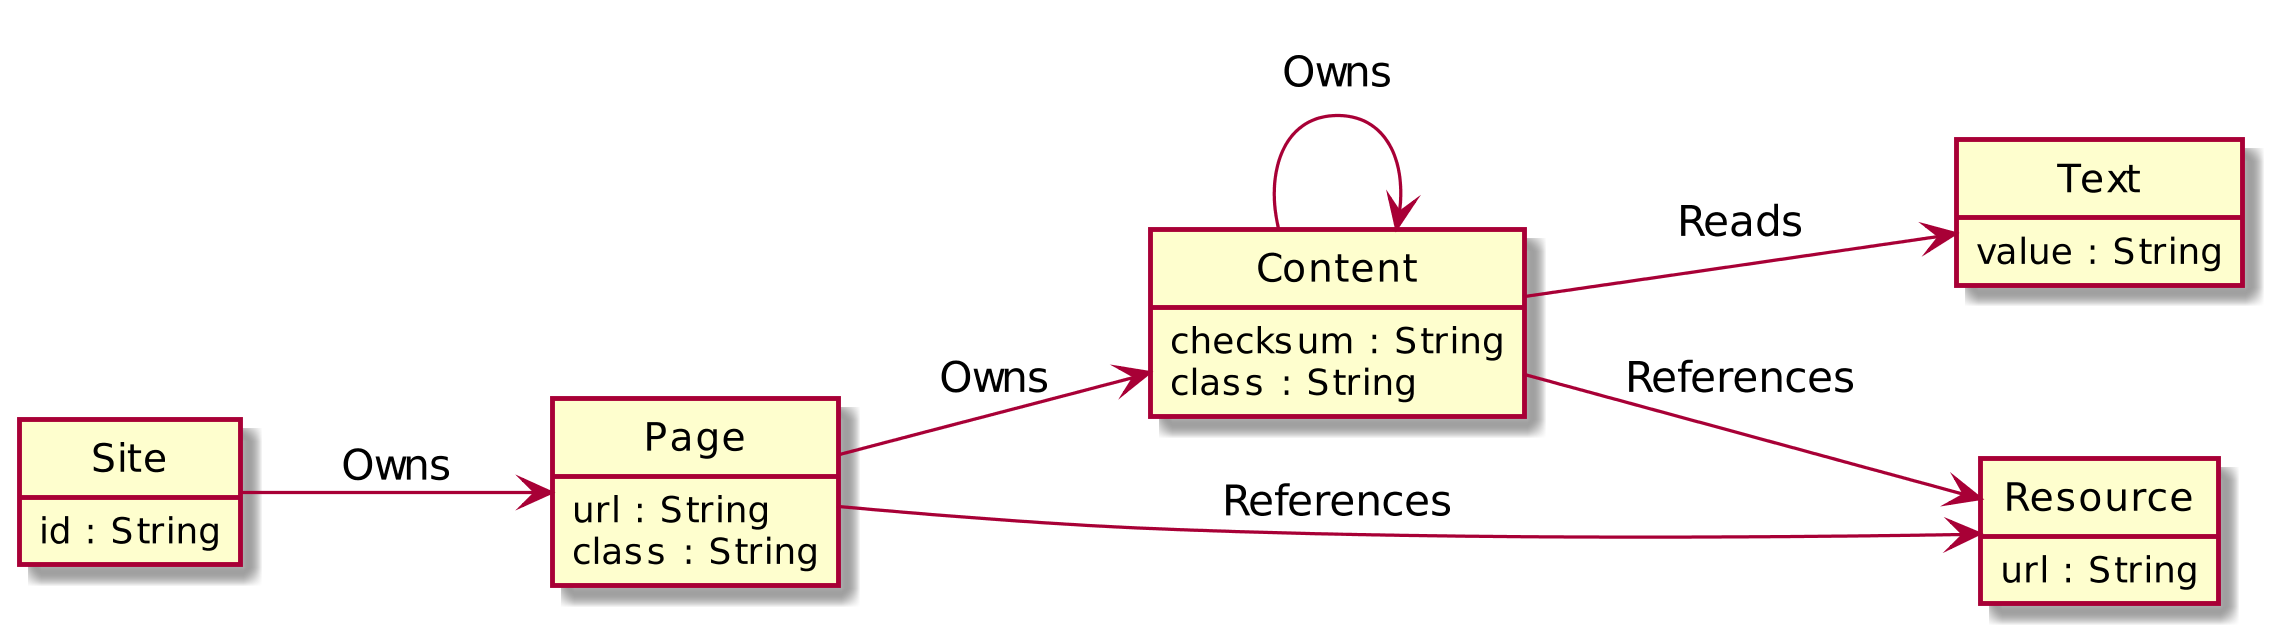
\includegraphics[width=\textwidth]{../resources/db-data-model/nodes.png}
                \caption{Übersicht der Nodes und ihrer Beziehungen}
                \label{image:dbDataModelOverview}
            \end{figure}

            \begin{figure}
                \centering
                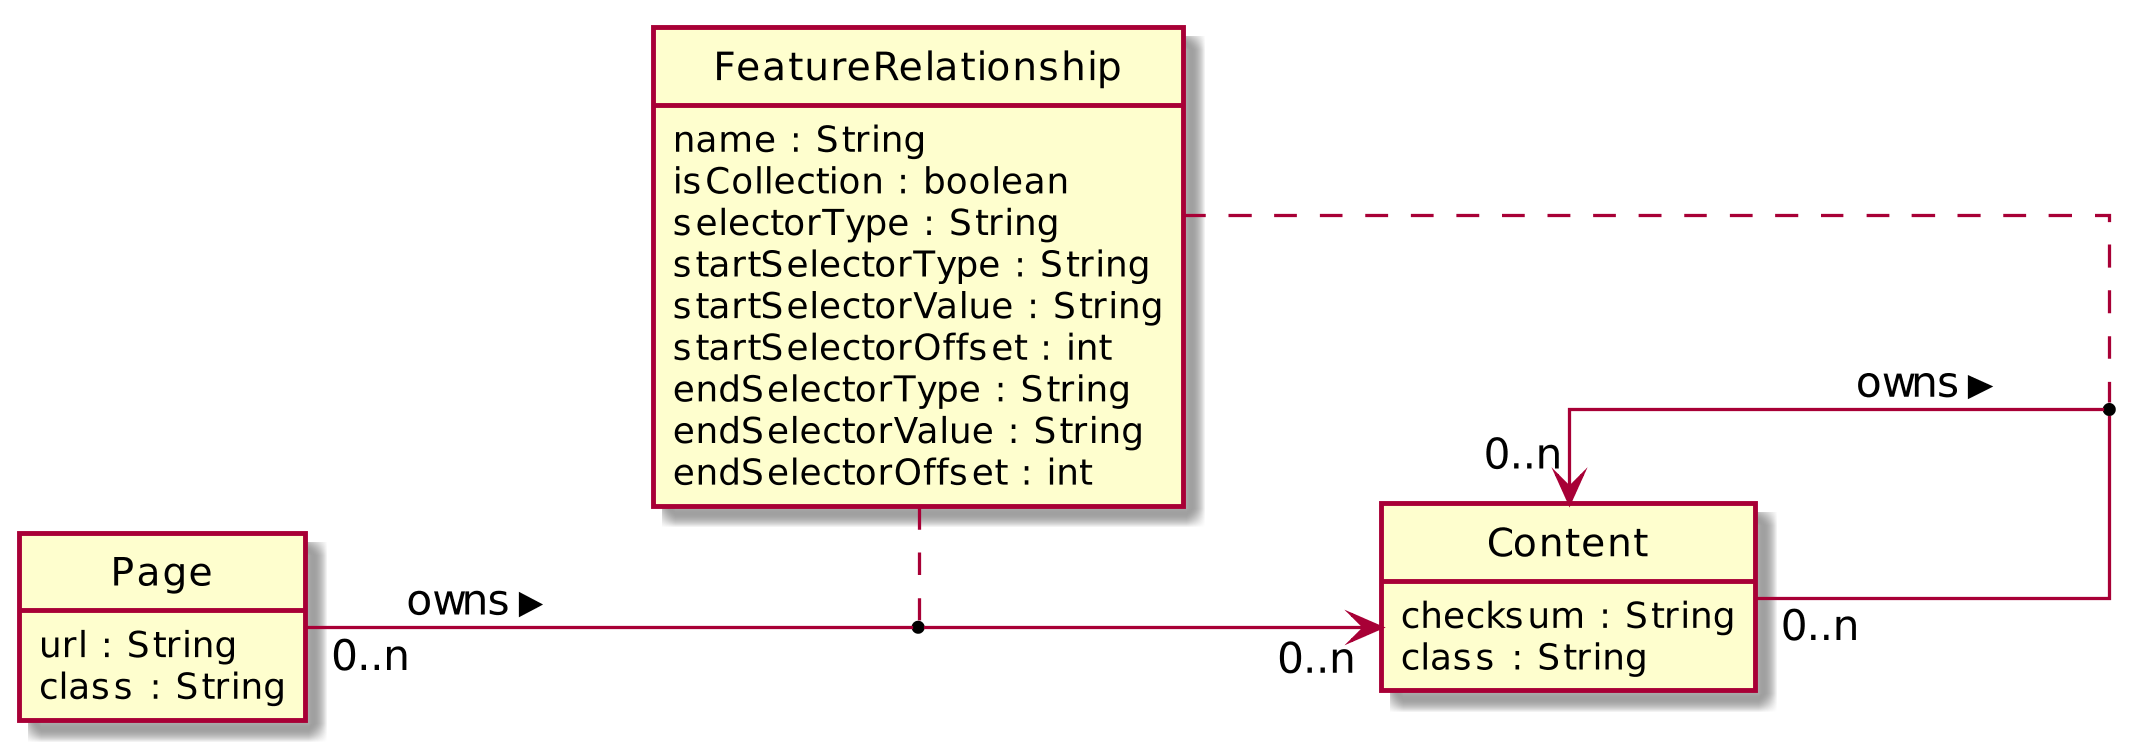
\includegraphics[width=\textwidth]{../resources/db-data-model/content-relationship.png}
                \caption{Content Features}
                \label{image:dbDataModelContentRelationship}
            \end{figure}

            \begin{figure}
                \centering
                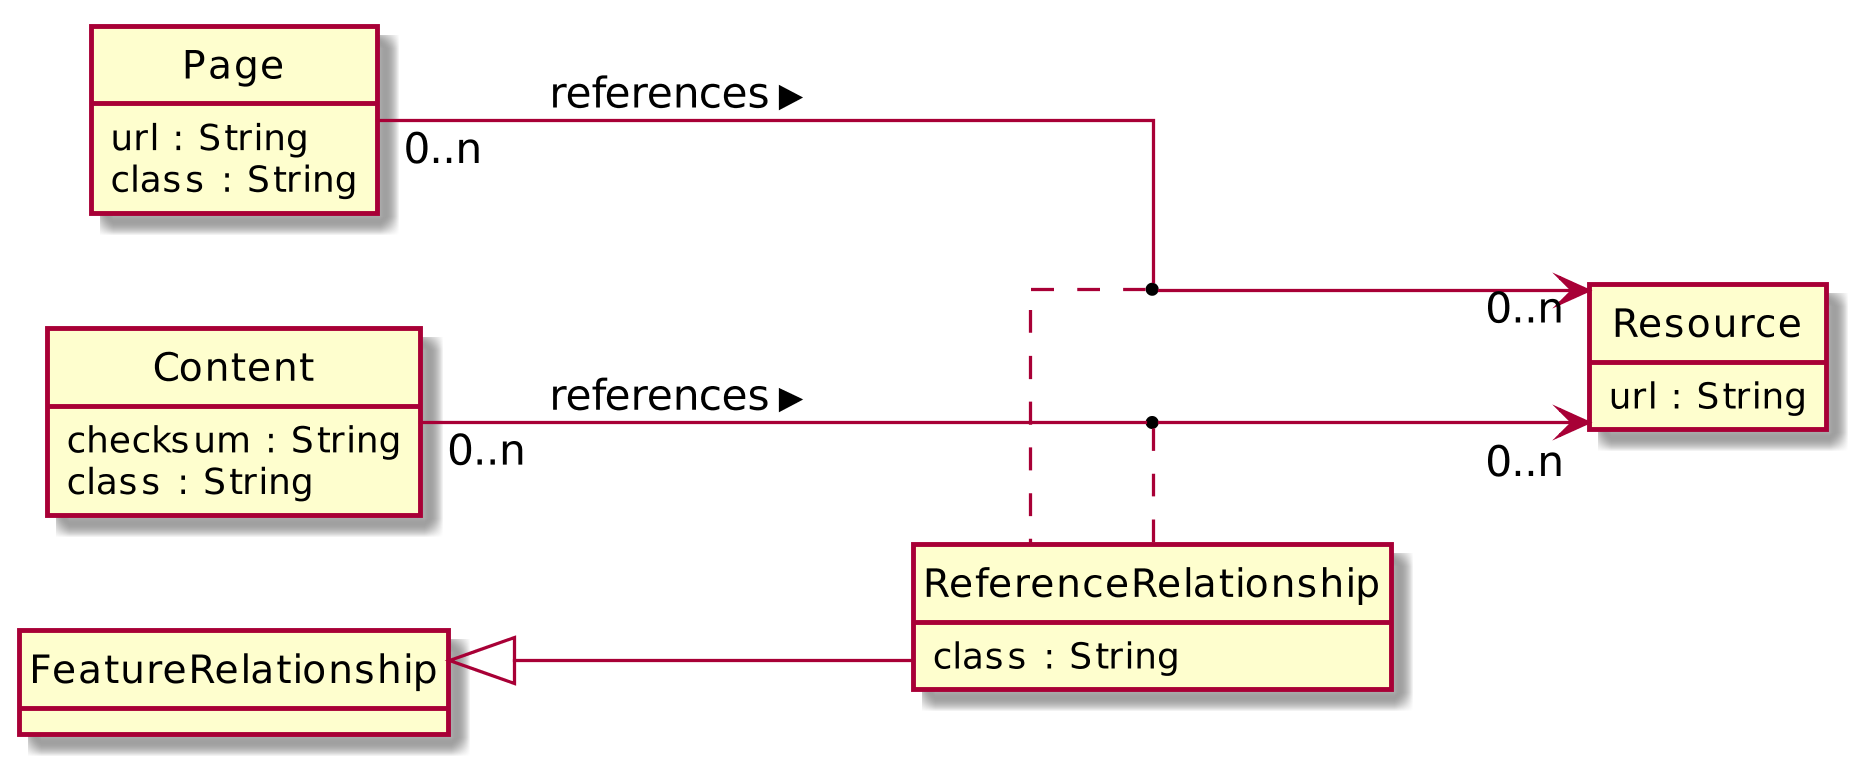
\includegraphics[width=\textwidth]{../resources/db-data-model/resource-relationship.png}
                \caption{Reference Features}
                \label{image:dbDataModelResourceRelationship}
            \end{figure}

        \subsection{Datenmodell Beispiel}
            \begin{figure}
                \centering
                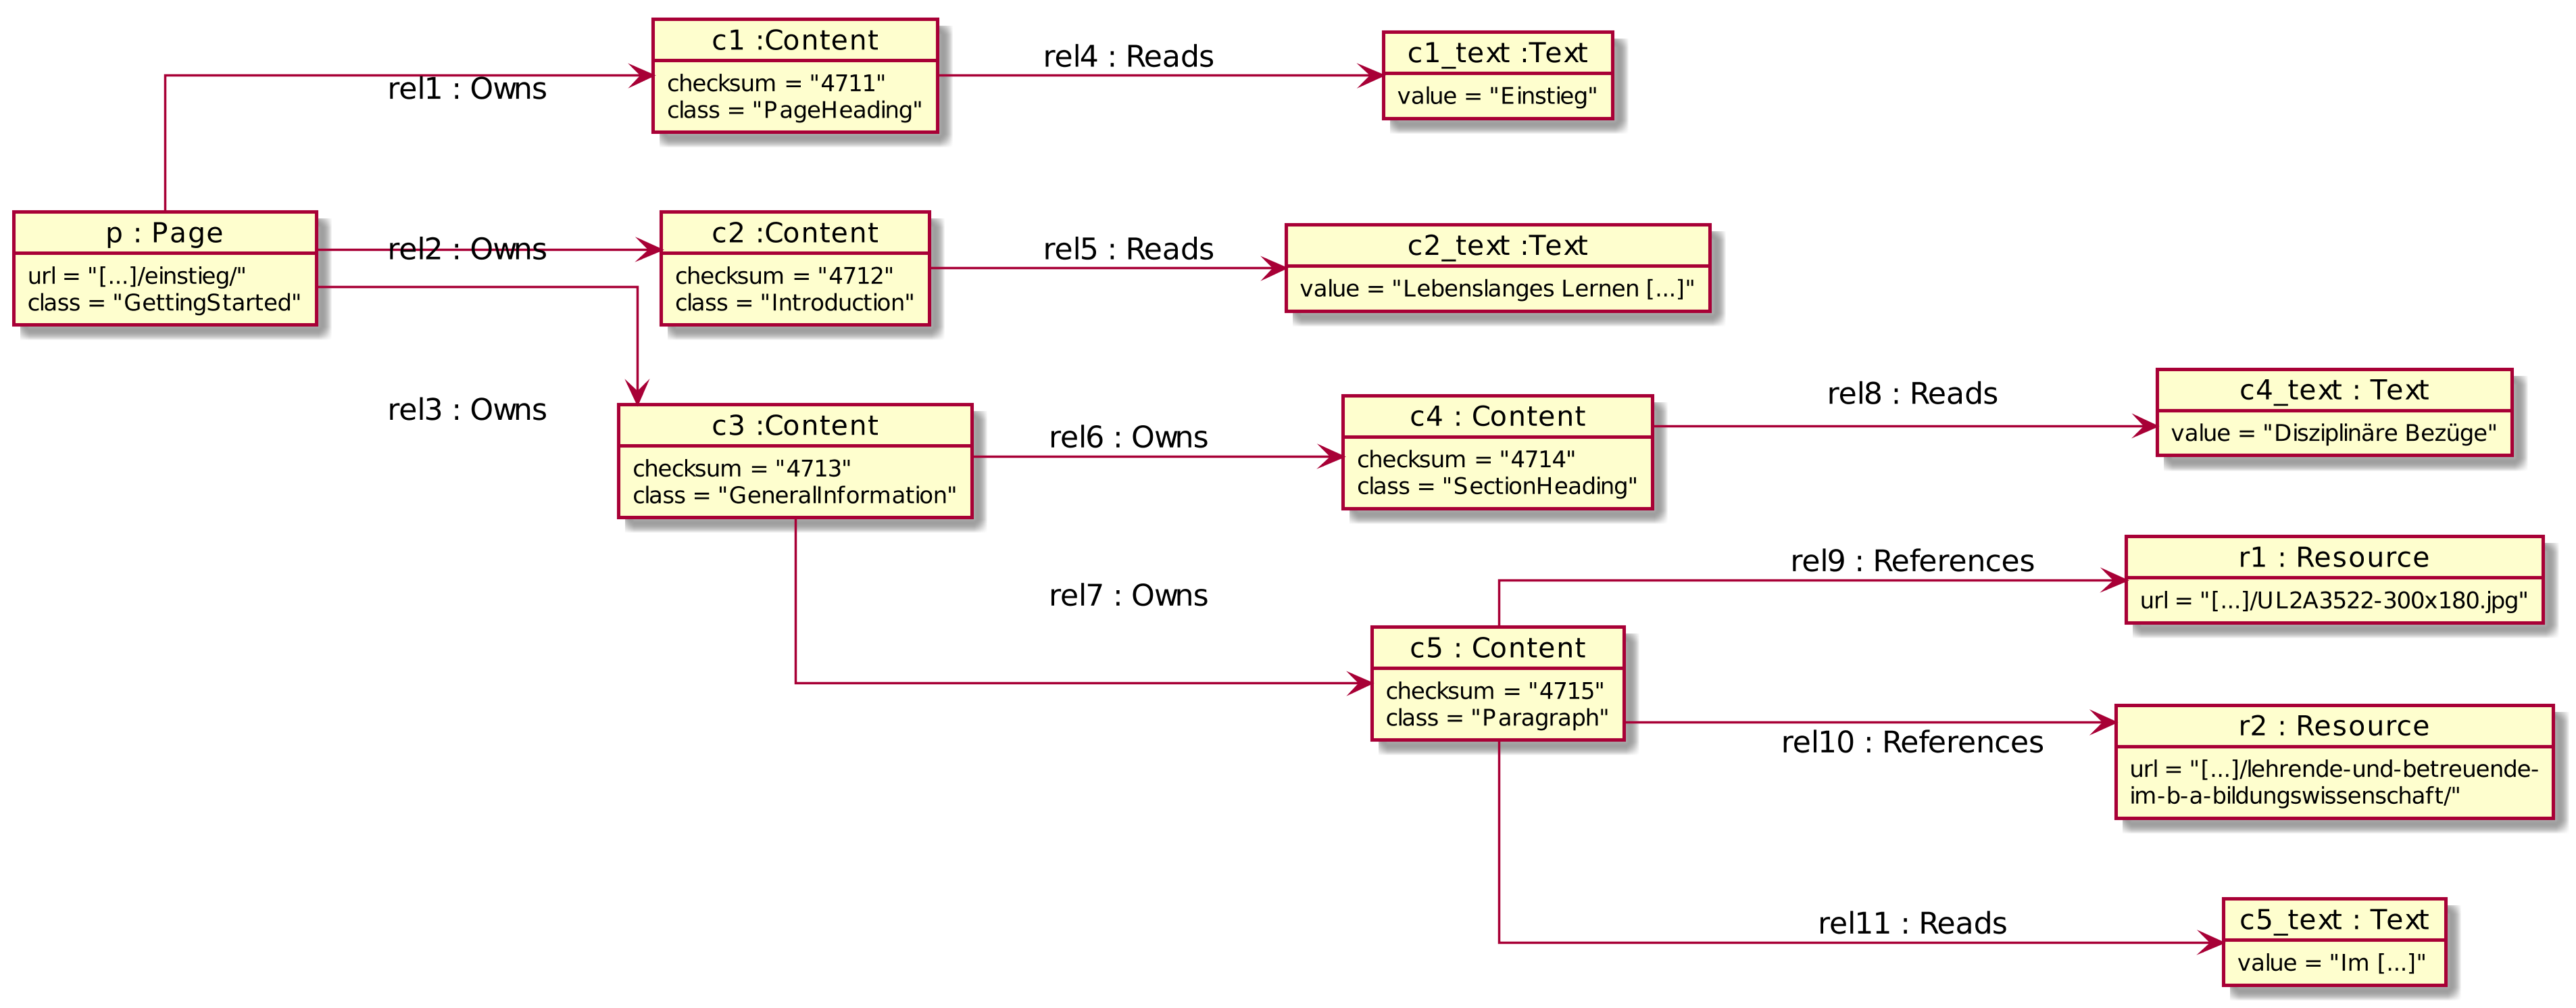
\includegraphics[width=\textwidth]{../resources/db-data-model/example/example.png}
                \caption{Beispiel}
                \label{image:dbDataModelExampleOverview}
            \end{figure}

            \begin{figure}
                \centering
                \begin{subfigure}{\textwidth}
                    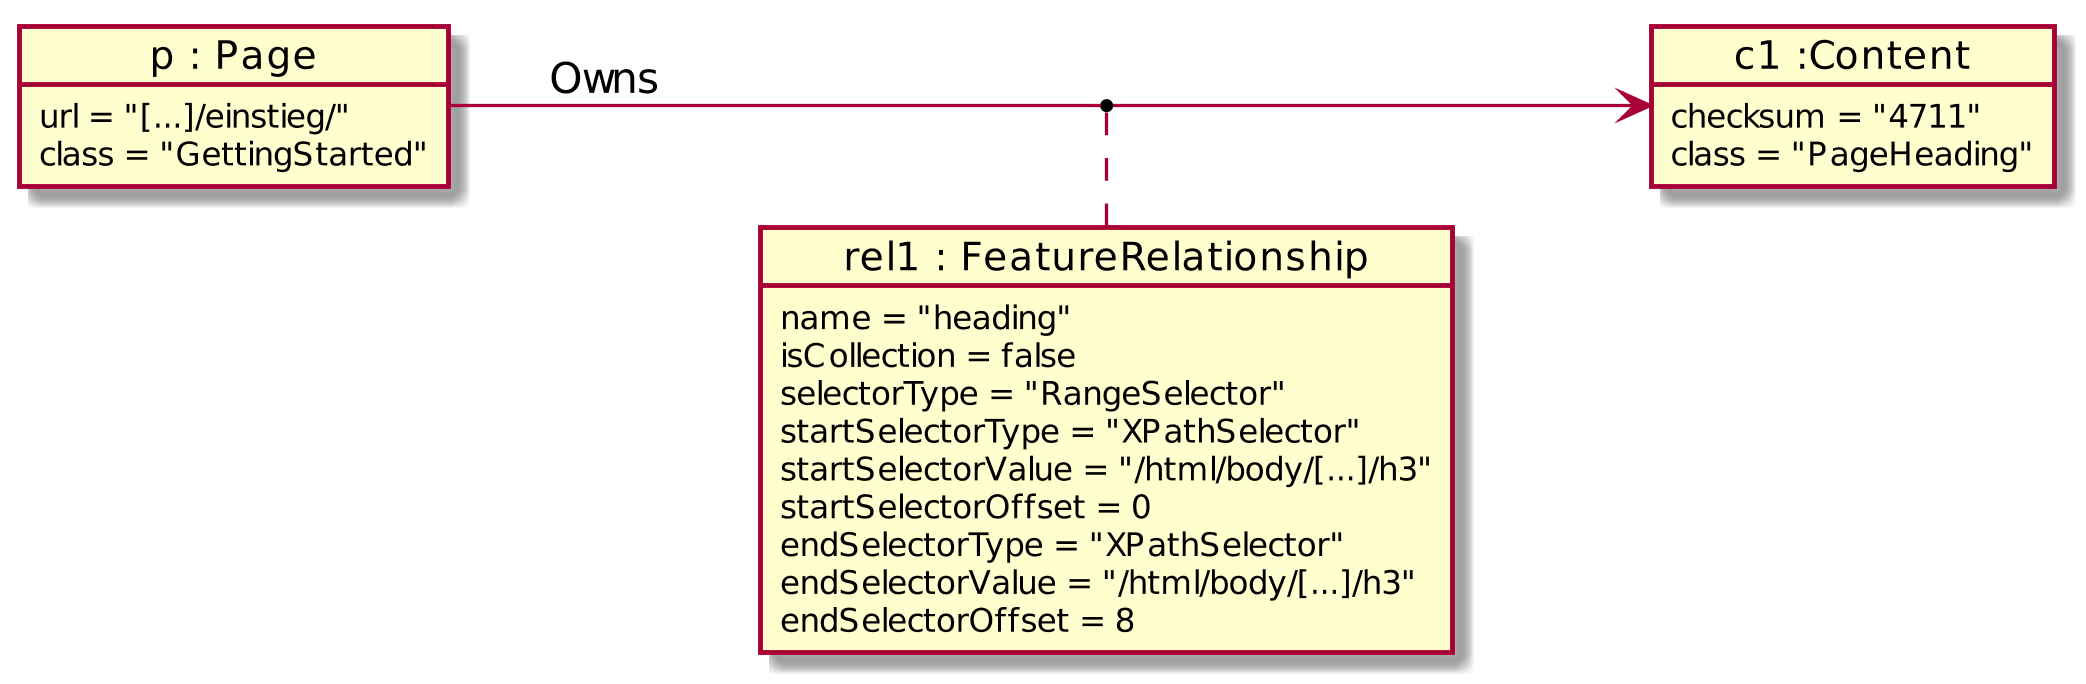
\includegraphics[width=\textwidth]{../resources/db-data-model/example/p-c1.png}
                    \subcaption{Rel 1}                    
                \end{subfigure}

                \begin{subfigure}{\textwidth}
                    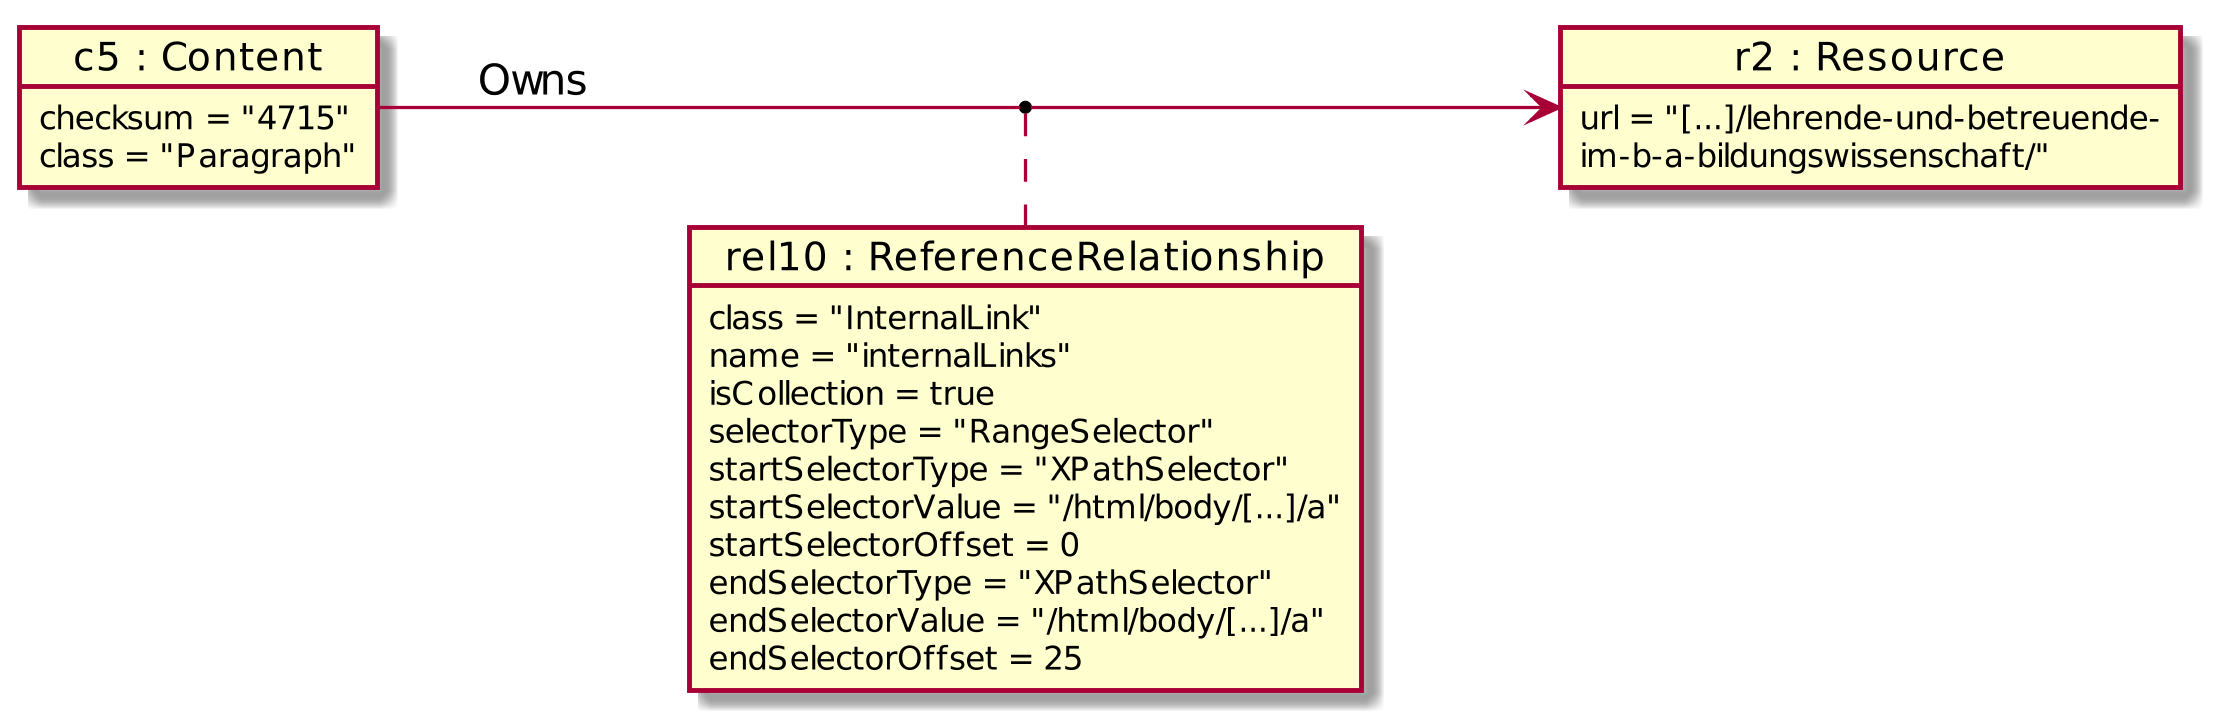
\includegraphics[width=\textwidth]{../resources/db-data-model/example/c5-r2.png}
                    \subcaption{Rel 2}                    
                \end{subfigure}
                \caption{Beziehungen}
                \label{image:dbDataModelExampleRelationships}
            \end{figure}

        \subsection{Classification Storage API}
            Wie werden die Daten in die DB geschrieben bzw. gelesen.

        \subsection{Was ist eine Seite}
            \begin{figure}
                \centering
                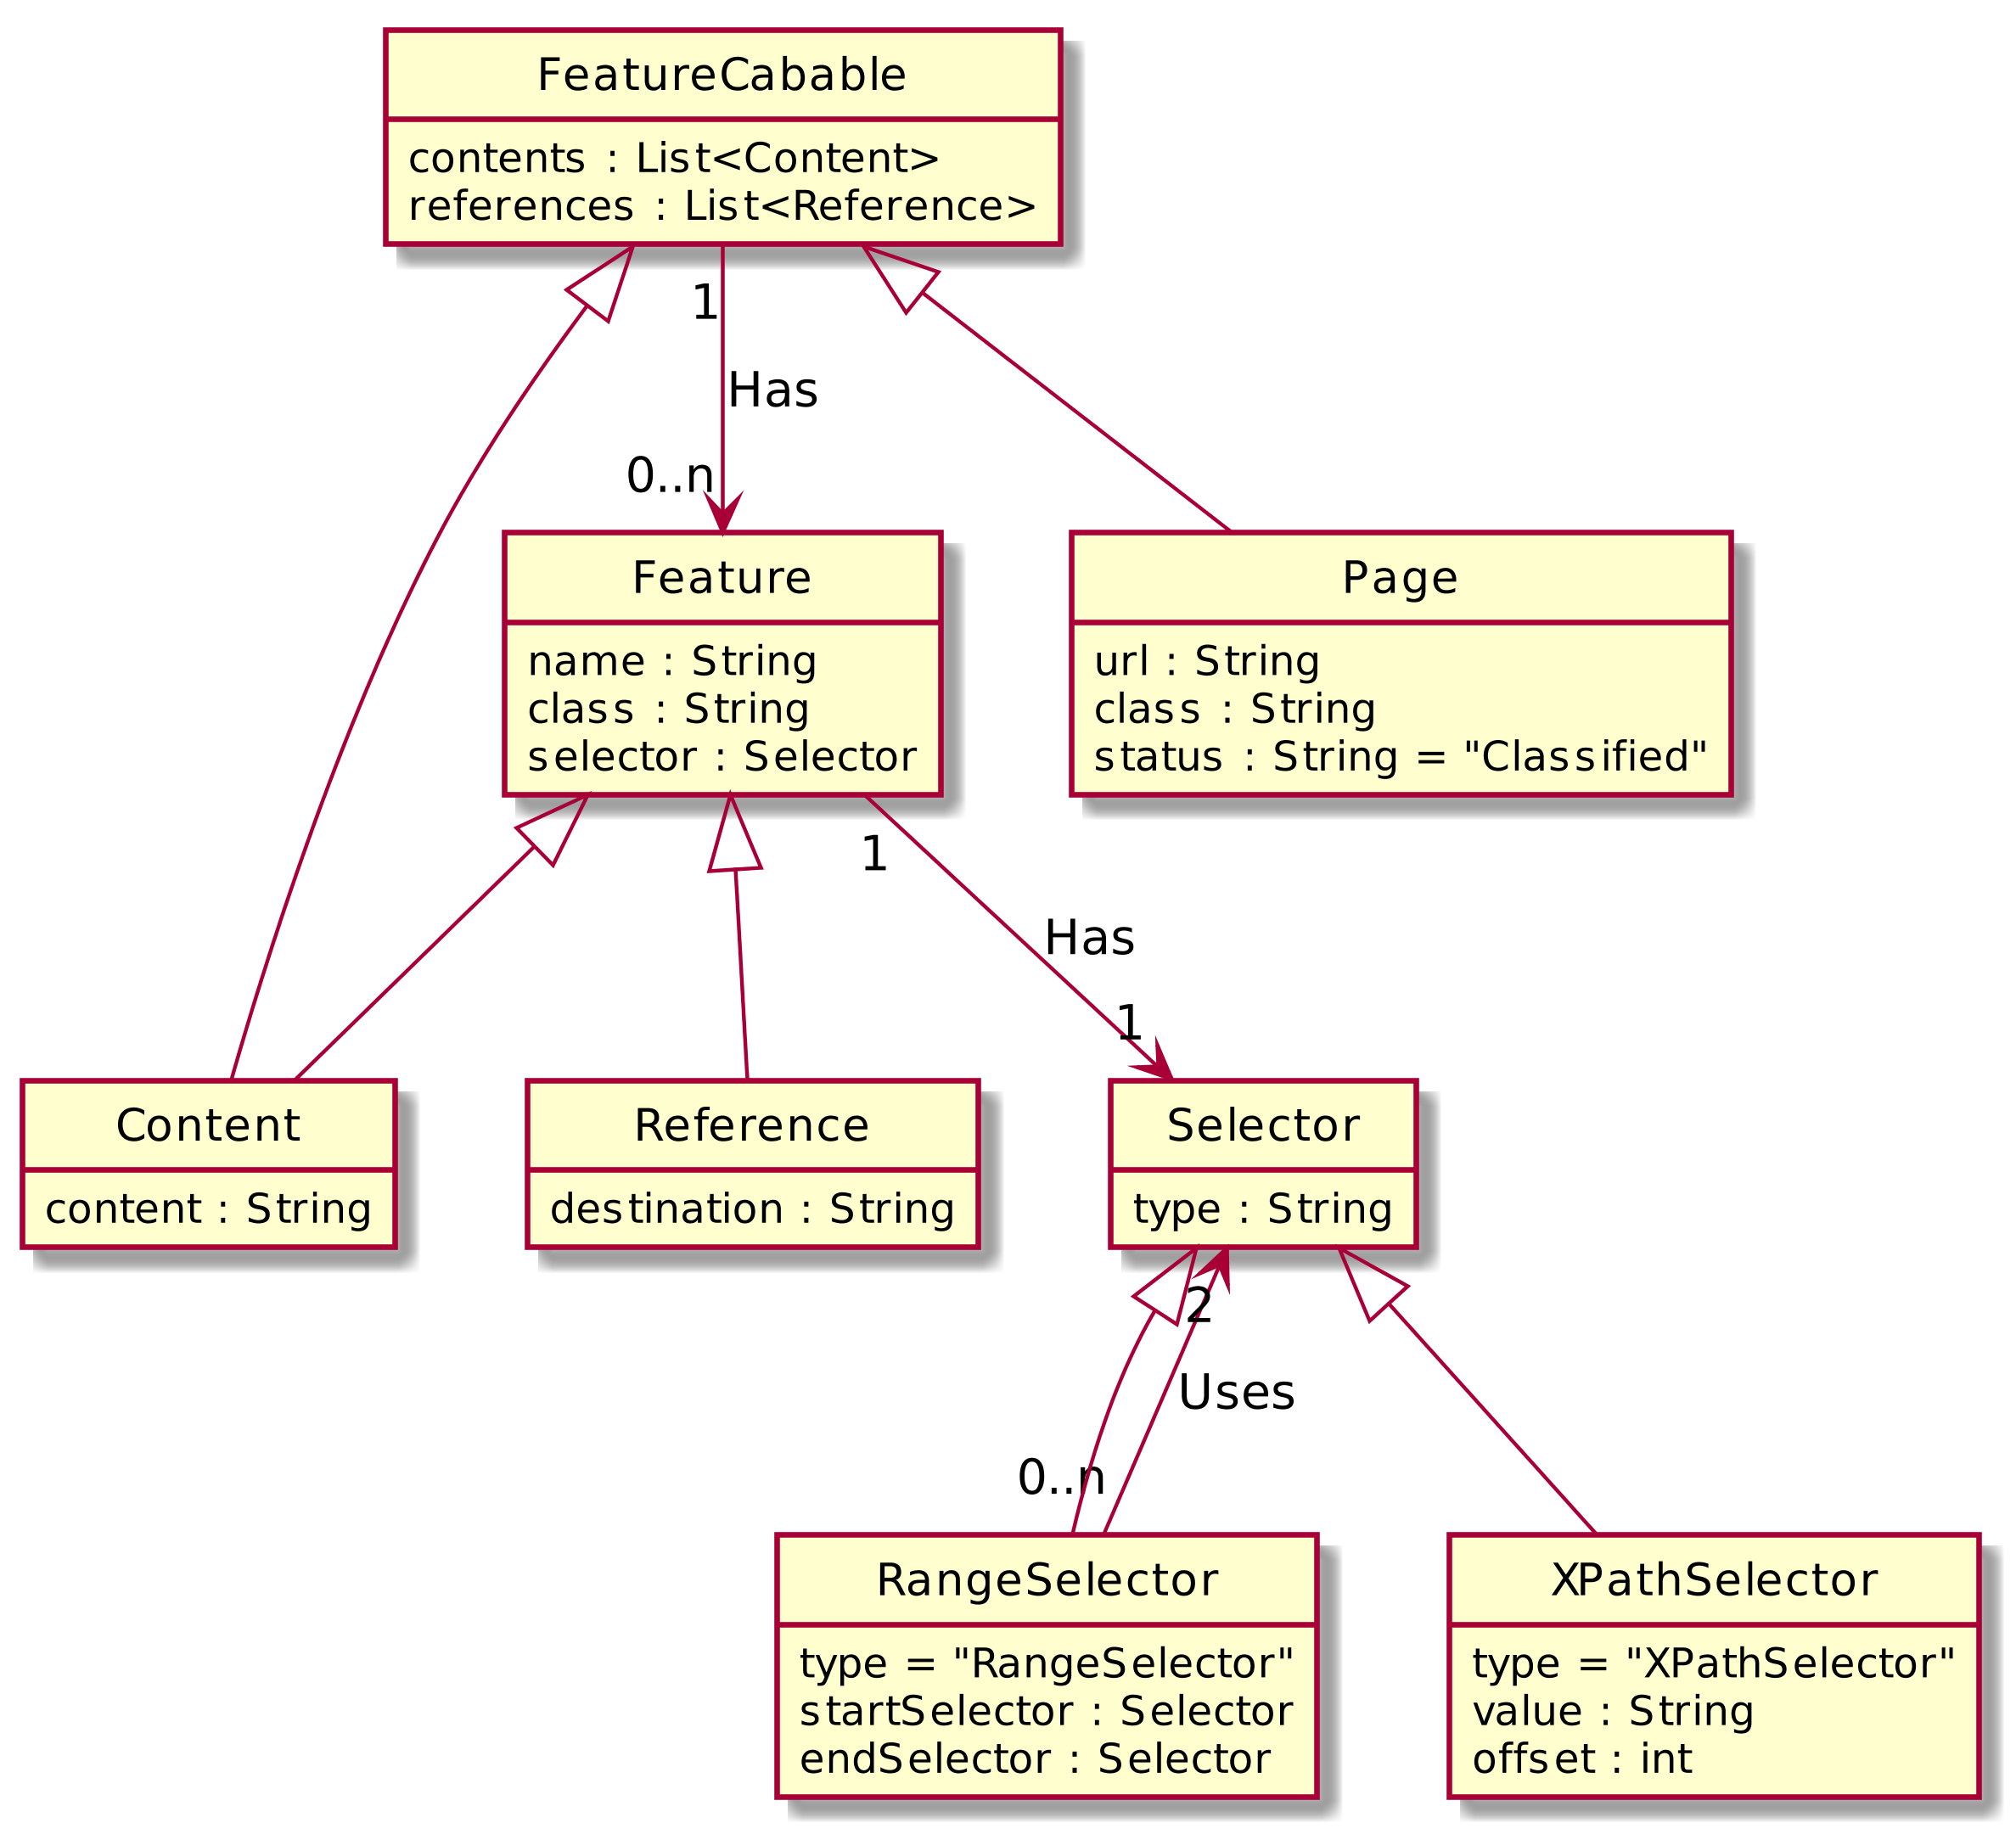
\includegraphics[width=\textwidth]{../resources/storage-api-data-model/page.png}
                \caption{Seite in der Storage API}
                \label{image:storageApiPageModel}
            \end{figure}
        
        \subsection{Algorithmus zum (initialen) ANLEGEN}
            \lstinputlisting[label=listing:storeClassification,caption=Algorithmus zum Speichern]{../resources/store-classification.code}

    \section{Annotation Service}
        \begin{table}[htb]
            \centering
            \begin{tabular}{|l|l|}
            \hline
            \textbf{Endpunkt}     & /pages/\{pageId\}\\
            \hline
            \textbf{Methode}      & GET\\
            \hline
            \textbf{Beschreibung} & Liefert Annotator Storage API version\\
            \hline
            \textbf{Status}       & 200\\
            \hline
            \textbf{Antwort}      & \{ ``name'': ``Annotator Store API'', ``version'': ``2.0.0'' \}\\
            \hline
            & \\
            \hline
            \textbf{Endpunkt}     & /pages/\{pageId\}/annotations\\
            \hline
            \textbf{Methode}      & GET\\
            \hline
            \textbf{Beschreibung} & Liefert alle Annotationen einer Seite\\
            \hline
            \textbf{Status}       & 200\\
            \hline
            \textbf{Antwort}      & \{ ``name'': ``Annotator Store API'', ``version'': ``2.0.0'' \}\\
            \hline
            \end{tabular}
            \caption{My caption}
            \label{my-label}
        \end{table}
        % Schnittstellenbeschreibung:
        % - Endpunkt
        % - Methoden
        % -- Input-Dokument
        % -- Status Codes der Antwort
        % -- Return Dokument für jede Antwort

    \section{Annotator Plugin}
    \section{Webanwendung}
    \section{WordPress Crawler}

    